\documentclass{article}
\usepackage[pdftex]{graphicx}
\author{M.Mancini,R.Modolo, S. Hess}

\title{Hyb 3D. Technical report and developer notes}
\newcommand{\br}{{\bf r}} 
\newcommand{\fu}{{\it future \,}}
\newcommand{\mk}{{\tt Makefile\,}}
\begin{document}
\maketitle
\begin{abstract}
  This document contains the description of the \textbf{hyb\_3D}
  code: its philosophy, its routines and the manual to implements new
  environments.
\end{abstract}

\section{The philosophy}

\section{The structure}

The structure of the code is such that a minimum number of files should be edited/created by the user. Namely, general parameters for the simulation are defined in {\sf defs\_parameters.F90}, a {\sf env\_}{\it name}{\sf .F90} file must be created in not already existing, and pointers to routines in this file may be set in {\sf environment.F90}.

\subsection{Module naming convention}
Because of FORTRAN limitations, modules and routines cannot share the same name. This issue was dodged by adding ``m$\_$'' in front of the module name. However, a better usage could be done of this mandatory prefix. Hence prefixes are now: \\
$\bullet$ ``defs\_'', if the module mainly contains structures or variable definitions.\\
$\bullet$ ``diag\_'', if the module is related to diagnostics.\\
$\bullet$ ``env\_'', if the module contains the environment of a given planet.\\
$\bullet$ ``atm\_'', for the modules containing the subroutines shared by the planet environement files (photoproduction, ionosphere,...). {\bf atm\_ modules should only be called by env\_ modules}.\\
$\bullet$ ``field\_'', if the module is related to fields.\\
$\bullet$ ``particle\_'', if the module is related to particles.\\
$\bullet$ ``m\_'', for the micellaneous modules which are directly related to the main program.\\
All other modules contains mostly general routines which cannot be classified into one of the groups mentioned above.
Note that in addition to hyb\_3d.F90, which contains the main program, initialisation.F90 and time\_schedule.F90, which do the initialization and the iterations have no prefix, as they can be understood as part of the main program. Figure 1 shows a summary of all the modules and the kind (Bloc) they belong to. Note that this division in blocs is not only related to the physical objects they deal with, but that modules in the same bloc are more closely related (through calls) than modules in different blocs.

%*********************************************
\begin{figure}[h]
\centering
\hspace{-1cm}
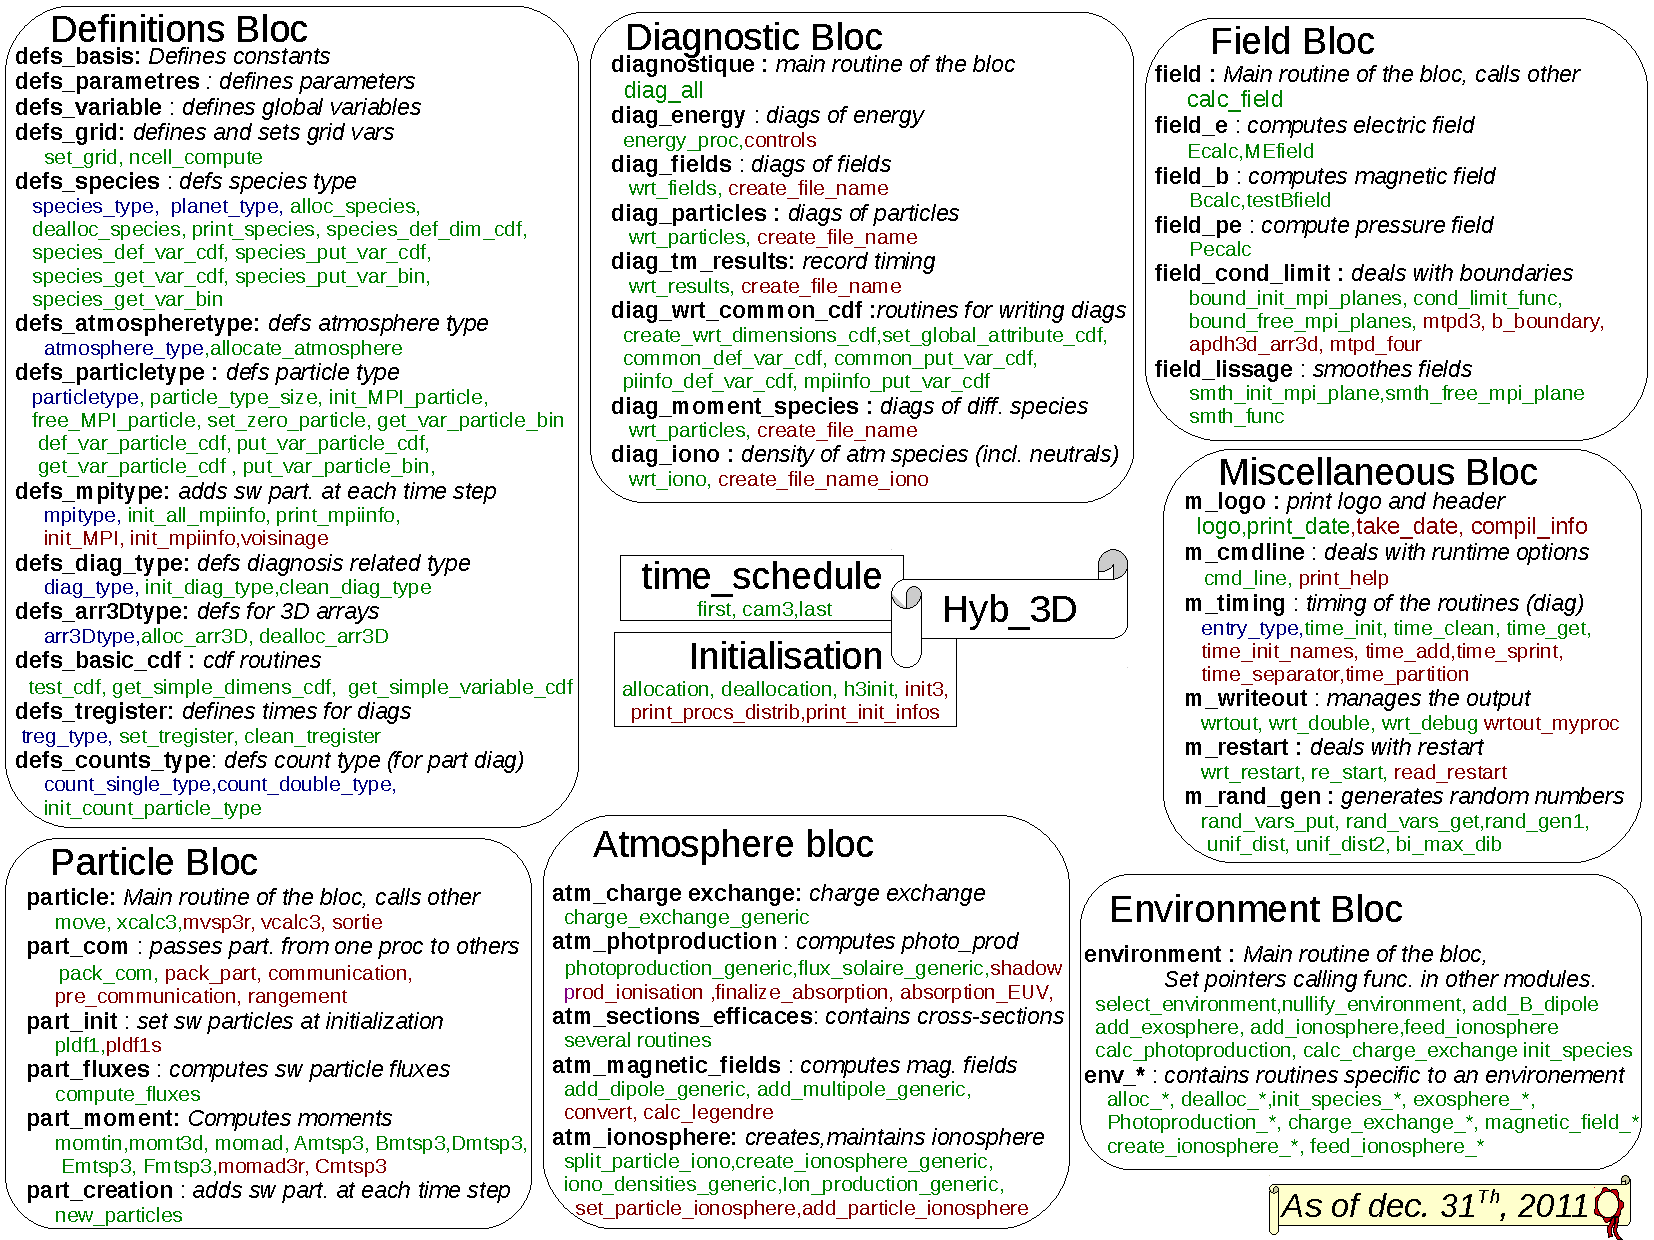
\includegraphics[width=\linewidth]{hybrid_str.pdf}
\caption{Organization of the modules, routines in the modules are shown in green for public ones and red for private ones. Data types are also shown in the module which defines them, in blue.}
\end{figure}
%*********************************************

\section{Defs\_parametre.F90}

This file define most of the parameters of the simulation which are not specifically related to the environment. In particular, all the parameters which can be modified through the command line are defined here.

\subsection{Space and time (relate them here)}
$\bullet$ {\sf ncx0,ncy0,ncz0}. Size of the grid, in cell number. Note that the code may automatically resize the grid so to be commensurable with the number of processes.\\
$\bullet$ {\sf gstep(3)}. Size of a cell, in units of the inertail length of the main ionic specie.\\
$\bullet$ {\sf dt}. Time step\\
$\bullet$ {\sf nhm}. Number of iterations\\

\subsection{IMF and Planet}
The IMF direction is defined with the spherical variables {\sf psi} (Z versus XY) and {\sf phi} (X versus Y). The module of the IMF is defined in the environment file.\\

The environment file which will be used depends on {\sf planetname}.

\subsection{Fields and Ionosphere additional settings}

Some particular settings can be set to describe how the ionosphere interacts we the surrounding plasma. These settings are defined in {\sf defs\_parametre.F90}:\\
$\bullet$ {\sf absorp\_surface}. If set to 1, the particles reaching the planet surface are absorbed, otherwise they are lost.\\
$\bullet$ {\sf t\_iono\_release}. Can be used to freeze the ionosphere up to a given time, for a smoother initialization.\\
$\bullet$ {\sf ipe}. Defines the polytropic law : 0 = adiabatic; 1 = isothermal; 2 = adiabatic in solar wind and hydrostatic in the ionosphere ($\gamma\propto 1/\log(density)$); 3= isothermal in solar wind and hydrostatic in the ionosphere.\\
$\bullet$ {\sf dn\_lim\_inf\_conduc}. Above this density (in simulation units, i.e. must be multiplied by the solar wind density to have physical units), the conductivity of the ionosphere is assumed to be infinity: the $v_i\times B$ term is set to $0$. Use this to cancel a abnormal diffusion of negative $E_y$ field in the ionosphere which leads to the ejection of a large part of the ionosphere.\\
$\bullet$ {\sf idisp, iresis}. Set to 1 to use dissipation or resistive terms in the electric field computation.\\
$\bullet$ {\sf resis}. Set the value of the resistivity.\\
$\bullet$ {\sf dmin}. Minimum density for the computation of the electric field.

\subsection{Optimization}

As the simulation box is a cube, with a planet or satellite in its center, some regions on the corners of the simulation box may not play any role in the simulation result (they just see an unperturbed flow of plasma). Moreover, if the planet/satellite as an ionosphere/exosphere, there will be more macroparticles close to it than in the corners of the simulation box. If the simulation box is splitted between the different process in sub-boxes of same sizes, this will lead to (1) processes processing more particles than others, (2) processes simulating nothing interesting. To limit this, it is possible to define a region of interest (ROI) in defs\_parametres.F90. This ROI must be defined manually, through 6 variables:\\
$\bullet$ y\_min, y\_max: define the position of the ROI in y, in fraction of the total box size in y (y\_min=0.33 and y\_max=0.67 correspond to a ROI occupying the central third of the box).\\
$\bullet$ z\_min, z\_max: define the position of the ROI in z, in fraction of the total box size in z.\\
$\bullet$ excess : define by how much the size of the box in the ROI must be shrinked (0 means no changes).\\
$\bullet$ excess\_part : allow to inject more particle in the ROI (0 means no changes).\\


\section{Environment.F90}
This module serves as an interface between the global part of the code and the code specific to the environment simulated. This is done through the definition of a few pointers to the function specific to the environment. This pointers are associated with functions which: (1) make computations specific to an environment, (2) fill the to structures which defines the property of the plasma flow ({\sf species} structure) and of the  exosphere/ionosphere/magnetic field/anything associated with the planet ({\sf atmosphere}).\\

To define an environment, a new {\sf env\_}{\it name}{\sf .F90} file must be created and the following pointers should be associated with routines in this file to enable the related physical processes:
\subsection{planet\_species $=>$}
This pointer must be associated with a routine which initializes the {\sf specie}s structure defined in {\sf defs\_species.F90}. 
\subsection{dealloc\_planet $=>$}
This pointer must be associated with a routine which deallocates arrays definied in the {\sf env\_}{\it name}{\sf .F90} file
\subsection{exosphere $=>$}
This pointer must be associated with a routine which computes the density of the neutral species in the exosphere.
\subsection{photoproduction $=>$}
This pointer must be associated with a routine which computes the photoproduction rates of some species. Note that if the cross-sections of the photoproduction reactions have previously been stored in the {\sf atmosphere} variable, this pointer can directly be associated with {\sf photoproduction\_generic} which is a generic function.
\subsection{charge\_exchange $=>$}
This pointer must be associated with a routine which implementes the charge exchange processes. Note that if the cross-sections of the charge exchange reactions are constant and have previously been stored in the {\sf atmosphere} variable, this pointer can directly be associated with {\sf charge\_exchange\_generic} which is a generic function.
\subsection{ionosphere $=>$}
This pointer must be associated with a routine which creates an ionosphere at initialization.
\subsection{b\_dipole $=>$}
This pointer must be associated with a routine which compute the internal magnetic field of the planet.
\subsection{feed\_production $=>$}
This pointer must be associated with a routine which computes the rates of ionization of the plasma through the simulation domain and create the corresponding macro-particles.

\paragraph{Important}
Does not change the number and the order of dummy arguments of the
subroutines. The procedure pointers are sensible to the dummy argument
list so if change the dummy argument order into {\tt m\_exo\_future.o}
you have to do that for all environment-dependent exosphere calculations.


\section{The Species structure}
This structure contains most of the information about the incident plasma flow and the obstacle. It should be filled in the routines associated to the {\sf planet\_species} pointer in {\sf environment.F90}. before the call to {\sf planet\_species}, the number of incident species {\sf ns} must be defined. This structure contains:

\subsection{Reference quantities}
These quantities are used to normalize the simulation variables.\\

$\bullet$ {\sf species\%ref\%density}.Physical density of reference, which normalizes density (m$^{-3}$)\\
$\bullet$ {\sf species\%ref\%c\_omegapi}. Ions inertial length, which normalizes lengths (km)\\
$\bullet$ {\sf species\%ref\%mag}. Magnetic Field, which normalizes fields (Tesla)\\
$\bullet$ {\sf species\%ref\%alfvenspeed}. Alfv\'en speed, which normalizes velocity (km.s$^{-1}$)\\
$\bullet$ {\sf species\%ref\%inv\_gyro}. Inverse of the gyrofrequency, which normalizes time (s).\\
$\bullet$ {\sf species\%ref\%maxabs}. maximum absorption length (km).\\

\subsection{Obstacle parameters}
$\bullet$ {\sf species\%planetname}. Name of the environment.\\
All the following distances or lengths are in simulation units:\\
$\bullet$ {\sf  species\%P\%centr}. Position of the planet center.\\
$\bullet$ {\sf  species\%P\%radius}. Radius of the planet.\\
$\bullet$ {\sf  species\%P\%r\_exo}. Radius of the exobase.\\
$\bullet$ {\sf  species\%P\%r\_lim}. Radius of the bottom limit of the ionosphere.\\
$\bullet$ {\sf  species\%P\%r\_iono}. Radius of the top limit of the ionosphere (when loaded explicitely).\\
$\bullet$ {\sf  species\%P\%speed}. Planet velocity.\\

\subsection{Incident plasma parameters}
$\bullet$ {\sf  species\%S(:)\%name}. Names of the incident species.\\
$\bullet$ {\sf  species\%S(:)\%ng}. Number of particles per cell for each species.\\
$\bullet$ {\sf  species\%S(:)\%vxs; ...\%vys; ...\%vzs}.  Directed velocities along x, y and z.\\
$\bullet$ {\sf  species\%S(:)\%percent}. Ratio of each species in the plasma flow. Total must be {\bf 1}.\\
$\bullet$ {\sf  species\%S(:)\%rcharge}. Species charges (ratio to the dominant specie).\\
$\bullet$ {\sf  species\%S(:)\%rmass}. Species masses (ratio to the dominant specie).\\
$\bullet$ {\sf  species\%S(:)\%rtemp}. Species temperatures (ratio to the dominant specie).\\
$\bullet$ {\sf  species\%S(:)\%betas}. $\beta$ of each species.\\
$\bullet$ {\sf  species\%betae}. $\beta$ of the electrons.\\
$\bullet$ {\sf  species\%S(:)\%rspeed}. Ratio $\frac{v_\|}{v_\perp}$ for each species.\\
$\bullet$ {\sf  species\%S(:)\%rvth}. Species thermal velocities (ratio to the dominant specie).\\
$\bullet$ {\sf  species\%S(:)\%rmds}. Species macroparticle weights (ratio to the dominant specie).\\
$\bullet$ {\sf  species\%S(:)\%qms}. Species charge over mass ratio (ratio to the dominant specie).\\
$\bullet$ {\sf  species\%S(:)\%vth1}. Species parallel velocities in simulation units.\\
$\bullet$ {\sf  species\%S(:)\%vth2}. Species perpendicular velocities in simulation units.\\
$\bullet$ {\sf  species\%S(:)\%sm}. Mass of the macroparticles of each species.\\
$\bullet$ {\sf  species\%S(:)\%sq}. Charge of the macroparticles of each species.\\

\subsection{Ionospheric plasma parameters}
$\bullet$ {\sf  species\%tempe\_ratio}. Temperature of the ionospheric electrons (ratio to the incident plasma electrons).\\
$\bullet$ {\sf  species\%viscosity}. Collision frequency of the ions in the ionosphere (in cm$^3$.s$^{-1}$).\\


\section{The Atmosphere structure}
The exophere is primarily defined through the use of the {\tt density\_exo} and {\tt prod\_pp} arrays defined in {\tt environment.F90}. From here, there are two ways of loading exospheric particles in the simulation: The first one is ``by hand'', through customized routines. You can use the {\tt exophere}, {\tt photoproduction}, {\tt ionosphere} and {\tt charge\_exchange} pointers in {\tt environment.F90} to call your routines. The second possibility is to use generic functions (those with the ``atm\_'' prefix) and an {\it atmosphere} structure. The following addresses the second option.\\


\subsection{Global environment variables}
The {\it atmosphere} structure is defined through the call, in {\sf environment.F90}, of a subroutine {\sf alloc\_}{\it planetname} which must exist in your {\sf env\_}{\it planetname}{\sf .F90} file. You must then define:\\
$\bullet$ the number of exospheric species (neutrals and ions): n\_species.\\
$\bullet$ the number of charge exchange reactions : n\_exc.\\
$\bullet$ the number of electron impact ionization reactions : n\_ei.\\
$\bullet$ the number of photoproduction reactions : n\_pp.\\
$\bullet$ the number of species produced by the photoproduction reactions (if two reactions produce the same ion) : n\_spe\_pp.\\
$\bullet$ the number of EUV wavelength for the photoproduction computations: nb\_lo.\\
$\bullet$ the number of photoproduction reactions whose rate does not depends on the wavelength : n\_pp\_freq\_fixed.\\

The {\it atmosphere} structure is obtained by calling:\\ {\sf allocate\_atmosphere(ncm,atmosphere,density,prod\_pp)}. Example:\\
\[
\begin{array}{l}
  \textsf{  atmosphere\%n\_species=7	      !number of exospheric species (neutral and ions)}\\
  \textsf{  atmosphere\%n\_pp=4    	      !number of photoproduction reactions}\\
  \textsf{  atmosphere\%n\_spe\_pp=3  	      !number of species obtained by photoproduction}\\
  \textsf{  atmosphere\%n\_pp\_freq\_fixed=0  !number of photoproduction reactions with fixed rates}\\
  \textsf{  atmosphere\%nb\_lo=37	      !number of wavelength in the EUV spectrum}\\
  \textsf{  atmosphere\%n\_exc=4	      !number of charge exchange photoreactions}\\
  \textsf{  atmosphere\%n\_ei=2	 	      !number opf electron impact reactions}\\
  \textsf{  call allocate\_atmosphere(ncm,atmosphere,density,prod\_pp)}
\end{array}
\]\\


Each species has then to be defined, one should precise:\\
$\bullet$ the species mass.\\
$\bullet$ the species charge.\\
$\bullet$ if the species opacity in EUV must be used (.TRUE. or .FALSE.).\\
$\bullet$ if the species must be load as ionospheric particle (.TRUE. or .FALSE.).\\
$\bullet$ the pointer to the photoproduction array for photoproduced species (only).\\
$\bullet$ the species name (no blank in front).\\
Examples:
\[
\begin{array}{l}
  \textsf{atmosphere\%species(1)\%name  = "O+        "}\\
  \textsf{atmosphere\%species(1)\%mass  = 16.\_dp}\\
  \textsf{atmosphere\%species(1)\%charge= one}\\
  \textsf{atmosphere\%species(1)\%opaque= .FALSE.}\\
  \textsf{atmosphere\%species(1)\%iono  = .TRUE.}\\
  \textsf{atmosphere\%species(1)\%prod  =$>$ prod\_pp(:,:,:,1)}\\
  \textsf{}\\
  \textsf{}\\
  \textsf{atmosphere\%species(2)\%name  = "O         "}\\
  \textsf{atmosphere\%species(2)\%mass  = 16.\_dp}\\
  \textsf{atmosphere\%species(2)\%charge= zero}\\
  \textsf{atmosphere\%species(2)\%opaque= .TRUE.}\\
  \textsf{atmosphere\%species(2)\%iono  = .FALSE.}
  \textsf{}\\
  \textsf{}\\
  \textsf{atmosphere\%species(3)\%name  = "H         "}\\
  \textsf{atmosphere\%species(3)\%mass  = 1.\_dp}\\
  \textsf{atmosphere\%species(3)\%charge= zero}\\
  \textsf{atmosphere\%species(3)\%opaque= .TRUE.}\\
  \textsf{atmosphere\%species(3)\%iono  = .FALSE.}
\end{array}
\]\\


\subsection{Photoproduction reactions}
The photoproduction has to be defined in the {\sf alloc\_}{\it planetname} subroutine. It is defined in the {\it atmosphere} structure, by setting pointers to the mother and daughter species. Example:
\[
\begin{array}{l}
  \textsf{  !O-$>$O+}\\
  \textsf{  atmosphere\%photo\_reactions(1)\%mother     =$>$ atmosphere\%species(2) !O species}\\
  \textsf{  atmosphere\%photo\_reactions(1)\%daughter   =$>$ atmosphere\%species(1) !O+ species}
\end{array}
\]\\
The fields atmosphere\%EUVFLX (EUV flux), atmosphere\%ion\_abs (absorption cross-section) and atmosphere\%ion\_react (ionization cross-section) will have to be filled before calling the subroutine {\sf photoproduction\_generic(Spe,ncm,gstep, s\_min\_loc,atmosphere)}, which computes the prod\_pp arrays in a generic way. Note that if these values (generally obtained through calls to routines of the {\sf atm\_sections\_efficaces.F90} module) are stored by {\sf alloc\_}{\it planetname}, you do not need to write a specific photoproduction routine and can compute the photoproduction rate by associating directly the photoproduction pointer to the {\sf photoproduction\_generic} routine in {\tt environment.F90}.\\

\subsection{Charge exchange reactions}
The charge exchange reactions have to be defined in the {\sf alloc\_}{\it planetname} subroutine. they are defined in the {\it atmosphere} structure, by setting pointers to the mother neutral and ion species as well as the charge/mass ratio of the mother ion specie and the cross-section of the reaction (if constant). Example:
\[
\begin{array}{l}
  \textsf{  !H +O+ -$>$H+ + O}\\
  \textsf{  atmosphere\%exc\_reactions(1)\%qsm        = one/16.\_dp}\\
  \textsf{  atmosphere\%exc\_reactions(1)\%ion        =$>$atmosphere\%species(1)}\\
  \textsf{  atmosphere\%exc\_reactions(1)\%neutral    =$>$atmosphere\%species(3)}\\
  \textsf{  atmosphere\%exc\_reactions(1)\%cross\_section = 9.E-20}
\end{array}
\]\\
The field atmosphere\%cross\_section will have to be filled before calling the subroutine {\sf charge\_exchange\_generic(nn,n2,pickup,qsm,irand, ijk,s\_p,v\_p,w,Spe,particule,atmosphere)}, which implementes the charge exchanges in a generic way. Note that if this valueis constant and is stored by {\sf alloc\_}{\it planetname}, you do not need to write a specific charge exchange routine routine and can compute the charge exchange rate by associating directly the charge\_exchange pointer to the {\sf charge\_exchange\_generic} routine in {\tt environment.F90}.\\


\subsection{Electron impact reactions}
The electron impact reactions have to be defined in the {\sf alloc\_}{\it planetname} subroutine. they are defined in the {\it atmosphere} structure, by setting pointers to the mother (neutral) and daughter (ion) species as well as the cross-section of the reaction defined by $\sigma=\sum_{i=1}^n \textsf{coeff}(i)*\ln(T_e(K))^{i-1}$. Example:
\[
\begin{array}{l}
  \textsf{  !O + e-$>$ O+}
  \textsf{  atmosphere\%ei\_reactions(2)\%ion        =$>$atmosphere\%species(1)}\\
  \textsf{  atmosphere\%ei\_reactions(2)\%neutral    =$>$atmosphere\%species(2)}\\
  \textsf{  atmosphere\%ei\_reactions(2)\%n          = 5}\\
  \textsf{  atmosphere\%ei\_reactions(2)\%coeff(1:5) = (/-1233.29,347.764,-37.4128,1.79337,-0.032277/)}
\end{array}
\]\\
The electron impact reactions are automatically implemented if defined in {\sf atmosphere}, without needing further declaration in {\sf environment.F90}.\\


\section{The Makefile}
The \mk is a gnu Makefile and permits to compile easily the {\tt
  quiet\_plasma} and {\tt diag} binaries.

\subsection{Compiler choice}
It contains the {\sf COMPILER} flag where you have to put the path
toward the mpi fortran.
Then there are three flags which permit to select the compile option
for anyone of the three compiler tested:
\begin{description}
\item[{\sf IFORTFLAG}] Compilation flags for intel fortran (tested
  with version 10.1 and 11.1).
\item[{\sf GFORTFLAG}] Compilation flags for gfortran (tested for
  versions $\ge$ 4.0).
\item[{\sf PGFORTFLAG}] Compilation flags for Portland Group fortran
  (work for version $\ge$ 10).
\end{description}
To select the good compiler flags you have to change the value of the
{\sf FFLAGS} variable accordingly with the compiler chosen.


The source files are compiled by "make" command. The corresponding
object files are listed in the \mk by respecting the dependencies between the modules.
At the moment the program structure and the object file list permits
to compile the program in parallel with two threads. So with the command
"make -j 2"  you can compile {\tt quiet\_plasma} very quickly.

\subsection{Compilation Options}
The {\tt quiet\_plasma} program have some compilation options
which enabling or not some {\it PREPROCESSOR MACROS} permits to
compile the program for some specific purposes.
\begin{description}
\item[{\sf HAVE\_TIMING}] Complete time analysis.
\item[{\sf HAVE\_NETCDF}] Read and Write of diagnostic files in NetCDF format.
\item[{\sf HAVE\_DEBUG}] Enable debug. For any called routine, the begin
  and the end are annotated. More controls on the quantities.
  Add also the good path to headers and libraries in the {\sf INC\_CDF}
  and {\sf LIB\_CDF} flags.
\item[{\sf HAVE\_DOUBLE\_PRECISION}] Use double precision real instead
  of simple precision.
\item[{\sf HAVE\_NO\_PLANET}] No planet is not considered, only the environment.
\item[{\sf HAVE\_WAVE\_TEST}] The input plasma is a Alfven wave. Use
  with {\sf HAVE\_NO\_PLANET}.
\item[{\sf HAVE\_MAXSIZEWRITE}] If in writing, the system have some
  limitation in the buffer size, then this option permits to write
  some big quantities (like particles) not at once.
\end{description}

To activate one of more of the compilation option add
{-DHAVE\_"option"} to the compilation flag in use.


\end{document}
